\section{Strings} 
Strings sind Arrys/Vektoren vom typ char. Mit Strings speichert man folglich längere Zeichenketten und benötigt \texttt{\#include<string>}. Dank überladener Operatoren haben Strings einige Zusatzfunktionen zu Vektoren.

\subsection{Initialisierung / Funktionen}
\begin{lstlisting}
	std::string text(3, 'u'); 	// {u, u, u}
	std::string name = "Cedric";
	name += " Renda";
	std::cout<< name = "Robin von Reding"; //false
	std::cout<< name = "Cedric Renda"; //true
\end{lstlisting}
\subsection{ASCII-Tabelle}
Werte vom Typ \texttt{int} und \texttt{char} lassen sich einfach konvertieren.
\begin{lstlisting}
	int i=97;
	char c=i;
	std::cout<<c; //Output: a
	c = 'A';
	i = c;
	std::cout<<i; //Output: A
\end{lstlisting}
Der Compiler geht dabei nach folgender Tabelle vor.
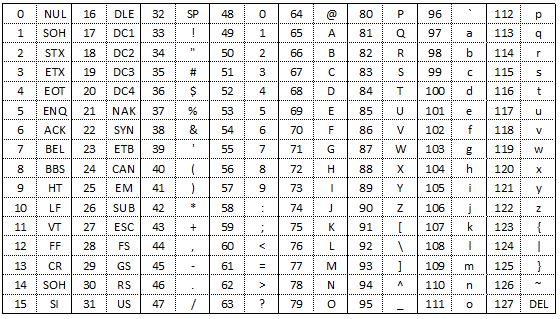
\includegraphics[width=0.24 \textwidth]{sections/ASCII-Tabelle}
\begin{tabular}{rlcrl}
	00-31:& NUL, ... & \quad & 32:& SPACE\\
	48-57:& 0-9& \quad &	65-90:& A-Z \\
	97-122:& a-z & \quad & 127:& DEL\\
\end{tabular}




